\documentclass[10pt]{beamer}
\usepackage{xcolor}

% ------------------------------------------------------------------------
% Carga de tu preámbulo personalizado (preamble.tex)
% Asegúrate de tenerlo en la misma carpeta.
% ------------------------------------------------------------------------
\usetheme[progressbar=frametitle]{metropolis}
\usepackage{appendixnumberbeamer}
\usepackage{fancyvrb}
\usepackage{booktabs}
\usepackage[scale=2]{ccicons}
\usepackage{pgfplots}
\usepgfplotslibrary{dateplot}
\usepackage{type1cm}
\usepackage{lettrine}
\usepackage{ragged2e}
\usepackage{xspace}
\newcommand{\themename}{\textbf{\textsc{metropolis}}\xspace}
\usepackage{graphicx} % Allows including images
\usepackage{booktabs} % Allows the use of \toprule, \midrule and \bottomrule in tables
\usepackage[utf8]{inputenc} %solucion del problema de los acentos.
\usepackage{xcolor}
\definecolor{LightGray}{gray}{0.9}

\usepackage{minted}
\usemintedstyle{tango}
\newcommand{\mypyfile}[1]{\inputminted[linenos=true, fontsize=\footnotesize, frame=lines, framesep=5\fboxrule,framerule=1pt]{python}{#1}}

\setminted[python]{breaklines,frame=lines,framesep=2mm,baselinestretch=1.2,bgcolor=LightGray,linenos, fontsize=\footnotesize} % obeytabs=true, tabsize=2, showtabs=true}

%%%%%%%%%%%%%%%%%%%%%%%%%%%%%%%%%%%%%%%%%%%%%%%%%%%%%%%%%%%%%%%%%%%%%%%%%%%%%%%%%%%%%%
\setbeamercolor{progress bar}{fg=blue!50!black,bg=white!50!black}
\setbeamercolor{title separator}{fg=red!50!black,bg=white!50!black}
\setbeamercolor{frametitle}{fg=white!80!black,bg=red!50!black}
\title[PCFI161]{Programaci\'on para F\'isica y Astronom\'ia}
\subtitle{Departamento de Física.}

\newcommand{\myfront}{
\author[PCFI161]{Corodinadora: C Loyola \\ Profesoras/es C Loyola / C Femenías / Y Navarrete / C Ruiz}
\institute[UNAB]{Universidad Andrés Bello}
\date{Primer Semestre 2025}
}

\titlegraphic{%
  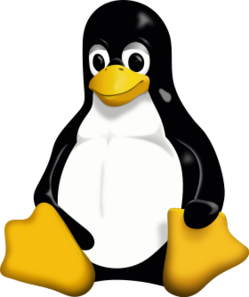
\includegraphics[width=.08\textwidth]{logo-tux.png}\hfill
  
\includegraphics[width=.3\textwidth]{logo-unab.png}\hfill
  
\includegraphics[width=.08\textwidth]{logo-python.png}
}

\makeatletter
\setbeamertemplate{title page}{
  \begin{minipage}[b][\paperheight]{\textwidth}
    \vfill%
    \ifx\inserttitle\@empty\else\usebeamertemplate*{title}\fi
    \ifx\insertsubtitle\@empty\else\usebeamertemplate*{subtitle}\fi
    \usebeamertemplate*{title separator}
    \ifx\beamer@shortauthor\@empty\else\usebeamertemplate*{author}\fi
    \ifx\insertdate\@empty\else\usebeamertemplate*{date}\fi
    \ifx\insertinstitute\@empty\else\usebeamertemplate*{institute}\fi
    \vfill
    \ifx\inserttitlegraphic\@empty\else\inserttitlegraphic\fi
    \vspace*{1cm}
  \end{minipage}
}
\makeatother


\makeatletter
\setlength{\metropolis@titleseparator@linewidth}{2pt}
\setlength{\metropolis@progressonsectionpage@linewidth}{2pt}
\setlength{\metropolis@progressinheadfoot@linewidth}{2pt}
\makeatother


\begin{document}

% ------------------------------------------------------------------------
% Portada de la Presentación
% ------------------------------------------------------------------------
\myfront{}

% ------------------------------------------------------------------------
% Slide 1: Título de la Sesión
% ------------------------------------------------------------------------
\begin{frame}
  \titlepage
  % Por ejemplo:
  % \title{Semana 4 - Sesión 1 (Sesión 7): Funciones en Python, Módulos y Paquetes}
\end{frame}

% ------------------------------------------------------------------------
% Slide 2: Índice / Tabla de contenidos
% ------------------------------------------------------------------------
\begin{frame}
  \frametitle{Resumen - Semana 4, Sesión 1 (Sesión 7)}
  \tableofcontents
\end{frame}

% ------------------------------------------------------------------------
% Configuración de bloques
% ------------------------------------------------------------------------
\metroset{block=fill}

% ----------------------------------------------------------------------------------------
% SECCIÓN 1: Introducción y Repaso de la Sesión Anterior
% ----------------------------------------------------------------------------------------
\section{Repaso y Contexto}


% ------------------------------------------------------------------------
% Slide 3: Repaso de las semanas previas y conexión con la sesión actual
% ------------------------------------------------------------------------
\begin{frame}{Repaso de Semanas Previas}
  \begin{itemize}
    \item \textbf{Semana 1:} Sintaxis básica, variables, tipos de datos y operadores.
    \item \textbf{Semana 2:} Estructuras de control: condicionales (\texttt{if-elif-else}), bucles (\texttt{for}, \texttt{while}).
    \item \textbf{Semana 3:} Definición y uso de funciones, alcance de variables, introducción a módulos.
    \item \textbf{Conexión:} Todos estos conceptos se integran en la sesión de hoy para crear aplicaciones más estructuradas y reutilizables.
  \end{itemize}
  \begin{block}{Ejemplo de integración}
    Un programa que calcula el área de figuras, valida datos y organiza el código en funciones y módulos.
  \end{block}
\end{frame}

% ------------------------------------------------------------------------
% Slide 4: Objetivos de la Sesión
% ------------------------------------------------------------------------
\begin{frame}{Objetivos de la Sesión}
  \begin{itemize}
    \item \textbf{Integrar} variables, operadores, estructuras de control y funciones en ejercicios prácticos.
    \item \textbf{Aplicar} la modularización mediante la creación y uso de módulos propios.
    \item \textbf{Desarrollar} habilidades para resolver problemas físicos y matemáticos usando Python.
    \item \textbf{Preparar} el terreno para proyectos colaborativos y el uso de paquetes externos.
  \end{itemize}
\end{frame}



% ----------------------------------------------------------------------------------------
% SECCIÓN: Ejercicios Guiados
% ----------------------------------------------------------------------------------------
\section{Ejercicios Guiados}

% ------------------------------------------------------------------------
% Ejercicio 1 (Fácil)
% ------------------------------------------------------------------------
\begin{frame}{Ejercicio 1: \hfill \textcolor{red}{$\clubsuit$} \\ Calcula el área de un triángulo}
  \begin{block}{Enunciado}
    \begin{itemize}
      \item Solicita la base y la altura de un triángulo en metros.
      \item Calcula el área usando la fórmula: \(A = \frac{1}{2} \times \text{base} \times \text{altura}\).
      \item Muestra el resultado con unidades.
    \end{itemize}
  \end{block}
  \textbf{Conceptos:} Variables, operadores, entrada/salida.\\
  \textbf{Física relevante:} Geometría básica.
\end{frame}

% ------------------------------------------------------------------------
% Ejercicio 2 (Fácil)
% ------------------------------------------------------------------------
\begin{frame}{Ejercicio 2: \hfill \textcolor{red}{$\clubsuit$} \\ Conversión de temperatura}
  \begin{block}{Enunciado}
    \begin{itemize}
      \item Solicita una temperatura en grados Celsius.
      \item Convierte a Fahrenheit usando la fórmula: \(F = C \times \frac{9}{5} + 32\).
      \item Muestra ambos valores.
    \end{itemize}
  \end{block}
  \textbf{Conceptos:} Variables, operadores, entrada/salida.\\
  \textbf{Física relevante:} Termodinámica básica.
\end{frame}

% ------------------------------------------------------------------------
% Ejercicio 3 (Fácil)
% ------------------------------------------------------------------------
\begin{frame}{Ejercicio 3: \hfill \textcolor{red}{$\clubsuit$} \\ Clasificador de números pares e impares}
  \begin{block}{Enunciado}
    \begin{itemize}
      \item Solicita un número entero.
      \item Indica si es par o impar usando condicionales.
    \end{itemize}
  \end{block}
  \textbf{Conceptos:} Condicionales (\texttt{if-else}), operadores.\\
  \textbf{Física relevante:} Lógica computacional.
\end{frame}

% ------------------------------------------------------------------------
% Ejercicio 4 (Intermedio)
% ------------------------------------------------------------------------
\begin{frame}{Ejercicio 4: \hfill \textcolor{red}{$\clubsuit$} \\ Calculadora de energía cinética}
  \begin{block}{Enunciado}
    \begin{itemize}
      \item Solicita masa (kg) y velocidad (m/s).
      \item Calcula la energía cinética: \(E_k = \frac{1}{2} m v^2\).
      \item Usa una función para el cálculo.
    \end{itemize}
  \end{block}
  \textbf{Conceptos:} Funciones, operadores, entrada/salida.\\
  \textbf{Física relevante:} Mecánica clásica.
\end{frame}

% ------------------------------------------------------------------------
% Ejercicio 5 (Intermedio)
% ------------------------------------------------------------------------
\begin{frame}{Ejercicio 5: \hfill \textcolor{red}{$\clubsuit$} \\ Simulador de caída libre}
  \begin{block}{Enunciado}
    \begin{itemize}
      \item Solicita altura inicial (m).
      \item Calcula el tiempo de caída usando \(t = \sqrt{2h/g}\), con \(g = 9.8\,m/s^2\).
      \item Muestra el resultado con unidades.
    \end{itemize}
  \end{block}
  \textbf{Conceptos:} Operadores, funciones, entrada/salida.\\
  \textbf{Física relevante:} Movimiento rectilíneo uniformemente acelerado.
\end{frame}

% ------------------------------------------------------------------------
% Ejercicio 6 (Intermedio)
% ------------------------------------------------------------------------
\begin{frame}{Ejercicio 6: \hfill \textcolor{red}{$\clubsuit$} \\ Tabla de conversión de metros a kilómetros}
  \begin{block}{Enunciado}
    \begin{itemize}
      \item Solicita un número entero \(n\).
      \item Imprime una tabla de conversión de los primeros \(n\) valores (1 a \(n\)) de metros a kilómetros.
    \end{itemize}
  \end{block}
  \textbf{Conceptos:} Bucles (\texttt{for}), operadores, entrada/salida.\\
  \textbf{Física relevante:} Unidades y conversiones.
\end{frame}

% ------------------------------------------------------------------------
% Ejercicio 7 (Intermedio)
% ------------------------------------------------------------------------
\begin{frame}{Ejercicio 7: \hfill \textcolor{red}{$\clubsuit$} \\ Validación de entrada: número positivo}
  \begin{block}{Enunciado}
    \begin{itemize}
      \item Solicita un número al usuario.
      \item Si el número es negativo, vuelve a pedirlo hasta que sea positivo.
      \item Muestra el número final.
    \end{itemize}
  \end{block}
  \textbf{Conceptos:} Bucles (\texttt{while}), validación de datos.\\
  \textbf{Física relevante:} Control de errores en mediciones.
\end{frame}

% ------------------------------------------------------------------------
% Ejercicio 8 (Difícil)
% ------------------------------------------------------------------------
\begin{frame}{Ejercicio 8: \hfill \textcolor{red}{$\clubsuit$} \\ Módulo de conversiones físicas}
  \begin{block}{Enunciado}
    \begin{itemize}
      \item Crea un módulo llamado \texttt{conversiones.py} con funciones para convertir:
        \begin{itemize}
          \item Metros a centímetros.
          \item Kilogramos a gramos.
          \item Segundos a minutos.
        \end{itemize}
      \item Importa el módulo y prueba cada función.
    \end{itemize}
  \end{block}
  \textbf{Conceptos:} Módulos, funciones, importación.\\
  \textbf{Física relevante:} Unidades físicas.
\end{frame}

% ------------------------------------------------------------------------
% Ejercicio 9 (Difícil)
% ------------------------------------------------------------------------
\begin{frame}{Ejercicio 9: \hfill \textcolor{red}{$\clubsuit$} \\ Calculadora de movimiento parabólico}
  \begin{block}{Enunciado}
    \begin{itemize}
      \item Solicita velocidad inicial (m/s) y ángulo (grados).
      \item Calcula el alcance máximo usando \(R = \frac{v_0^2 \sin(2\theta)}{g}\).
      \item Implementa la fórmula en una función y muestra el resultado.
    \end{itemize}
  \end{block}
  \textbf{Conceptos:} Funciones, operadores, módulos (\texttt{math}).\\
  \textbf{Física relevante:} Cinemática de proyectiles.
\end{frame}

% ------------------------------------------------------------------------
% Ejercicio 10 (Difícil)
% ------------------------------------------------------------------------
\begin{frame}{Ejercicio 10: \hfill \textcolor{red}{$\clubsuit$} \\ Clasificador de temperaturas usando módulos}
  \begin{block}{Enunciado}
    \begin{itemize}
      \item Crea un módulo \texttt{clima.py} con una función que recibe una temperatura en Celsius y retorna “Frío”, “Templado” o “Caliente” según el valor.
      \item Importa el módulo y prueba la función con diferentes valores.
    \end{itemize}
  \end{block}
  \textbf{Conceptos:} Módulos, condicionales, funciones.\\
  \textbf{Física relevante:} Clasificación de estados térmicos.
\end{frame}


% ----------------------------------------------------------------------------------------
% SECCIÓN 6: Conclusiones y Próximos Pasos
% ----------------------------------------------------------------------------------------
\section{Conclusiones}


% ------------------------------------------------------------------------
% Slide 23: Síntesis y Reflexión Final
% ------------------------------------------------------------------------
\begin{frame}{Síntesis de la Sesión}
  \begin{itemize}
    \item \textbf{Consolidamos:} el uso integrado de variables, operadores, condicionales, bucles y funciones.
    \item \textbf{Aplicamos:} la modularización y reutilización del código mediante módulos propios.
    \item \textbf{Resolvimos:} problemas físicos y matemáticos con Python, conectando teoría y práctica.
    \item \textbf{Preparamos:} el camino para el trabajo colaborativo y el uso de librerías externas.
  \end{itemize}
  \begin{block}{Habilidad adquirida}
    Capacidad para estructurar programas en Python de forma clara, eficiente y reutilizable.
  \end{block}
\end{frame}


% ------------------------------------------------------------------------
% Slide 25: Cierre y Motivación
% ------------------------------------------------------------------------
\begin{frame}
  \huge{\centerline{¡Excelente trabajo!}}
  \vspace{0.5cm}
  \normalsize
  \begin{itemize}
    \item Guarda tus avances y comparte dudas en el foro.
    \item Explora la documentación oficial de Python y experimenta con nuevos módulos.
    \item ¡Sigue practicando y colaborando!
  \end{itemize}
\end{frame}

\end{document}

